\documentclass[conference]{IEEEtran}
\IEEEoverridecommandlockouts
% The preceding line is only needed to identify funding in the first footnote. If that is unneeded, please comment it out.
\usepackage{cite}
\usepackage{amsmath,amssymb,amsfonts}
\usepackage{algorithmic}
\usepackage{graphicx}
\usepackage{textcomp}
\usepackage{xcolor}
\def\BibTeX{{\rm B\kern-.05em{\sc i\kern-.025em b}\kern-.08em
    T\kern-.1667em\lower.7ex\hbox{E}\kern-.125emX}}
    
% my packages

\usepackage[ruled,vlined,linesnumbered]{algorithm2e}
\usepackage{tikz}
\usepackage{pgfplots}
\usepgfplotslibrary{groupplots}
\pgfplotsset{compat=1.17} 
\usepackage[caption=false]{subfig}
% \usepackage[ngerman]{babel}
% \usetikzlibrary{decorations.pathreplacing,calligraphy,backgrounds}

% for bucket img
\usetikzlibrary{shapes.arrows,chains}
\usepackage{babel}
\usetikzlibrary{decorations.pathreplacing,calligraphy,backgrounds}
% \renewcommand\familydefault{\sfdefault} 
% \listfiles


% debug
\pagestyle{plain}

% 1. label of graph
% 2. picture
% 3. ref
% 4. perf on spiedie
% 5. host supported sketch

% the batches sync

\title{gpupaper}
\author{kchiu }
\date{May 2021}

\begin{document}
\maketitle
% \begin{multicols}{2}
\section{Introduction}
[to do]
\section{Background}
\subsection{GPU}
The Graphics Processing Unit (GPU) provides much higher instruction throughput and memory bandwidth than the CPU within a similar price and power envelope\cite{b1}. While the CPU is designed to excel at executing a few tens of these threads in parallel, the GPU is designed to excel at executing thousands of them in parallel\cite{b1}\cite{b2}. Threads are grouped into blocks(1, 2 or 3 dimensional), and blocks are organized into a grid(also 1, 2 or 3 dimensional). A thread block may contain up to 1024 threads and the GPU schedules and executes threads of the same block in groups of 32 parallel threads called warps\cite{b1}. Threads of a warp can only run in the same Streaming Multiprocessor (SM) and they must execute one common instruction in lockstep. Branch divergence occurs if the threads of a warp execute disjoint code paths, which will reduce the overall throughput, but different warps are free to execute common or disjoint code paths. 


\subsection{Global Memory}

The largest device memory is global memory, which has high memory throughput when the warps can coalesce the adjacent memory accesses.Because one physical memory transaction can actually access a tile of data. And when an instruction tries to access the global memory, if the physical addresses of different data are close enough that some transactions can actually access several addresses. [For devices of compute capability 6.0 or higher, the concurrent accesses of the threads of a warp will coalesce into a number of transactions equal to the number of 32-byte transactions necessary to service all of the threads of the warp.]  For example, if a warp plans to load a sequence of 32 4-byte integers, it may only need 4 32-byte memory transactions. However, if the 32 integers are stored on the random places among a large memory area, they are unlikely to be close to each other and can not be coalesced, so the 32 accesses may need 32 memory transactions. In this situation, each transaction transfers 32 bytes data and only 4 bytes are useful, the throughput is divided by 8. In order to achieve the peak performance, the data should also be at least 32-byte aligned[add more here]. 
% on a GPU with 1024-bit memory bus width, and the 32 memory accesses are coalesced into one. 
CUDA assumes that the device memories are weakly-ordered, that is the order of one thread writes data to memory is not guaranteed to be the same as the order in which the data is observed by another thread. For example, if thread A writes 1, 2, 3 to the global memory one by one, thread B may observes that A writes 2 at first. A memory function is needed to enforce the ordering. 
\subsection{Hash Function}
QSketch[to do] assumes that there is already a hash function that can map the input data to uniform distribution. It has a default hash function and several build-in hash functions, and the users can also define their own hash functions if it is necessary. Some user-defined hash functions may be slow or can not execute on GPU, but this won't reduce the performance. Because hash functions usually are independent and can execute simultaneously, so the time complexity of hash is still O(1).

\subsection{Sketch}
\begin{algorithm}
\DontPrintSemicolon
\caption{Sketch algorithm}
\SetKwProg{Fn}{Function}{}{end}
\SetKw{KwRet}{return}
\SetKwFunction{FnInsert}{insert}
\SetKwFunction{FnSearch}{search}
% \SetKwArray{HashTable}{table}
$table[n][m] \longleftarrow 0$\;
% \HashTable{n}{m}$ \longleftarrow 0$\;
\Fn()
{\FnInsert{key}}
{
    \For{$i\leftarrow 0$ \KwTo $m$}{
        $id \leftarrow hash(i, key) \% n$
        $table[id][i]$++
    }
}

\Fn()
{\FnSearch{key}}
{
    $count \leftarrow MAX\_INTEGER$\;
    \For{$i\leftarrow 0$ \KwTo $m$}{
        $id \leftarrow hash(i, key) \% n$
        % table[id][i]++
        $count \leftarrow min(count, table[id][i])$
    }
    \KwRet $count$\;
}
\end{algorithm}

A sketch is a data structure which can record the frequencies of elements. In the algorithm, n is a large number and the specific value of n is dependent on the input data size. The larger n will consume more memories and it should be more accuracy. However, m is a small number and should not be changed. 
Since the sketch doesn't need to store the element itself, it can receive elements as many as possible without increasing the memory usage.  
% Parallel sketch
In order to improve the performance of insert() and search(), it is not odd to implement a parallel version of sketch. However the parallel sketch is still limited by the low computer power of CPU and narrow memory bandwidth of host memory. 

\subsection{Related Work}

% hash map can't store lots of distinct elements on device.
Some hash tables for GPU have one atomic operation or one global memory access on average for each operation. The feature of hash table that needs to store the elements themselves makes hash table must consume a lot of device memory when storing a large number of different elements. On current GPUs, the insertion performance of hash tables can reach more than 1000Mops/s. And a GPU with approximately 16GB of memory to can only store up to 2000M 8-byte pairs, where both Key\_T and Mapped\_T of the pair are 4-byte integers. If it keep inserting different elements into the hash table, the GPU will usually run out of memory in less than 2 seconds. Even if some GPUs have much larger device memory (e.g. 48GB), the insertion can only last about 6 seconds. And disregarding these GPUs may have higher insertion performance because they have higher computing power and memory bandwidth. For hash tables of CPU, this is not a serious problem because they usually have much lower insertion performance and much larger memory. For a server with 256 GB of memory, a hash table may only have an insert performance of about 100Mops/s. The insert operation takes about 320 seconds to run out of memory, which is approximately 180 times longer than the hash tables of GPU.
% sketches suffer the random access
The sketches for GPU do not consider the characteristics of GPU memory and thus directly port CPU-specific algorithms to the GPU platform, preventing peak insertion and lookup performance. They focus more on improving accuracy than on insertion, deletion and searching performance. The several atomic functions and global memory accesses are not coalesced, and they will load lots of unused data which will reduce the overall memory throughput. The performance of sketch is greatly limited by the memory bandwidth so the sketches will experience a low performance on GPU.

\subsection{contribution}
We propose a new heterogeneous sketch, q-sketch, which has higher performance than other sketches and can still achieve the same accuracy. We implement the q-sketch and compare the performance and accuracy with other sketches.  
\section{QSketch}
\subsection{Thread Sketch}
\begin{algorithm}
    \DontPrintSemicolon
    \caption{Thread Sketch algorithm}
    \SetKwProg{Fn}{Function}{}{end}
    \SetKw{KwRet}{return}
    \SetKw{Kwin}{in}
    \SetKwFunction{FnInsert}{insert}
    \SetKwFunction{FnSearch}{search}
    % \SetKwArray{HashTable}{table}
    $table[n * m] \longleftarrow 0$\;
    % \HashTable{n}{m}$ \longleftarrow 0$\;
    \SetKwFor{ParallelForEach}{parallel for each}{do}{endfor}
\Fn(){\FnInsert{keys}}
{
    \ParallelForEach{$key$ \Kwin $keys$}
    {
      \For{$i\leftarrow 0$ \KwTo $m$} 
        {
            $id \leftarrow hash(i, key) \% n$\;
            atomic\_add($table[i * n + id]$, 1)\;
        }
    }
}
\Fn(){\FnSearch{keys, counts}}
{
    \ParallelForEach{$key$ \Kwin $keys$, $count$ \Kwin $counts$, }
    {
        $count \leftarrow MAX\_INTEGER$\;
      \For{$i\leftarrow 0$ \KwTo $m$}{
            $id \leftarrow hash(i, key) \% n$
            % table[id][i]++
            $count \leftarrow min(count, table[i * n + id]$
        }
    }
}

\end{algorithm}

% Naive implementation (sketch v0)
In this implementation, the threads of each warp load a group(32) of keys and each thread will handle one of them. It will invoke $m$ hash functions, and it also needs $m$ atomic increment for each insertion and $m$ global memory accesses for each searching. This kind of implementation of sketch is very straightforward and is the basement of other sketches with higher accuracy. However, this sketch implementation may not fully take advantage of the high memory bandwidth of GPU. The main reason is that the sketch tries to increase or access the count variables on $m$ random places, which suffers a low memory throughout due to the underlying CUDA memory architecture and the memory access instructions. The 32 threads in a warp are in a lock step and they will execute the 32 atomic instructions or random memory accesses simultaneously for $m$ times. The 32 random memory transactions are not likely to coalesced because they are too far form each other, and there will be 32 transactions for most situations. In each warp, it will need about $m x 32$ 32-byte memory transactions in total for every 32 operations and each of them will need $m$ global memory access or atomic operations on average. If the count variables are 4-byte integers, there are only 4 useful bytes for each 32-byte memory transaction, and the throughput is divided by 8 in theory.[to do :show the comparison of performance between random access and sequential access]

Things can be more serious while comparing sketch with Hash Map, because Hash Map usually only needs one memory access, but the sketch needs 3($m = 3$) or more memory accesses. That's why the sketch libraries are often slower than Hash Map libraries. This feature of the sketch greatly drops the performance, especially for the heterogeneous implementation.

Figure \ref{fig:thread_perf_m_0.5} shows the performance for $m = 1, 2, and 3$. For the large date set, the insertion and searching performance of $m = 2$ is reduced by $\frac{1}{2}$ compared to $m = 1$ and the performance of $m = 3$ is reduced by $\frac{2}{3}$ compared to $m = 1$. This indicates that the memory accesses are not coalesced for most operations.
\begin{figure}
    \centering
    \subfloat[Insert Performance for Different m\label{1i}]{
        \resizebox{0.48\columnwidth}{!}{
            \begin{tikzpicture}%[scale = 0.48]
                % \label{fig:thread_perf_m_0.5}
                \begin{semilogxaxis}[
                    % title={Insert Performance for Different m},
                    xlabel={Work Load},
                    ylabel={Insert Performance (M operations/s)},
                    legend pos=north east,
                    xmajorgrids=true,
                    ymajorgrids=true,
                ]
                    \addplot table[x = WorkLoad, y = m1_insert] {data/qsketch/perf_m_0.5_r.dat};
                    \addlegendentry{m == 1}
                    \addplot table[x = WorkLoad, y = m2_insert] {data/qsketch/perf_m_0.5_r.dat};
                    \addlegendentry{m == 2}
                    \addplot table[x = WorkLoad, y = m3_insert] {data/qsketch/perf_m_0.5_r.dat};
                    \addlegendentry{m == 3}
                \end{semilogxaxis}
            \end{tikzpicture}
        }
    }
    ~
    \hfill
    \subfloat[Search Performance for Different m\label{1s}]{
        \resizebox{0.48\columnwidth}{!}{
            \begin{tikzpicture}%[scale = 0.48]
            \begin{semilogxaxis}[
                % title={Search Performance for Different m},
                xlabel={Work Load},
                ylabel={Search Performance (M operations/s)},
                legend pos=north east,
                xmajorgrids=true,
                ymajorgrids=true,
            ]
                \addplot table[x = WorkLoad, y = m1_search] {data/qsketch/perf_m_0.5_r.dat};
                \addlegendentry{m == 1}
                \addplot table[x = WorkLoad, y = m2_search] {data/qsketch/perf_m_0.5_r.dat};
                \addlegendentry{m == 2}
                \addplot table[x = WorkLoad, y = m3_search] {data/qsketch/perf_m_0.5_r.dat};
                \addlegendentry{m == 3}
            \end{semilogxaxis}
        \end{tikzpicture}
        }
    }
    \caption{Performance for Different m}
    \label{fig:thread_perf_m_0.5}
\end{figure}

% And it is hard to cache the random accesses in l2 cache[to do]
\subsection{Warp Sketch}

\begin{algorithm}
    \DontPrintSemicolon
    \caption{Warp Sketch algorithm}
    \SetKwProg{Fn}{Function}{}{end}
    \SetKw{KwRet}{return}
    \SetKw{Kwin}{in}
    \SetKw{KwStep}{step}
    \SetKwFunction{FnInsert}{insert}
    \SetKwFunction{FnSearch}{search}
    $table[p * w] \longleftarrow 0$\;
    $\_shared\_ mask\_table[H] \longleftarrow generate\_hash\_mask(H)$\;
    \SetKwFor{ParallelForEach}{parallel for each}{do}{endfor}
\Fn(){\FnInsert{keys}}
{
    \ParallelForEach{$key$ \Kwin $keys$}
    {
    %   \For{$i\leftarrow 0$ \KwTo $m$} 
    %     {
            \If{$thread_index == 0$}{
                $hv \leftarrow hash(key)$\;
                $id \leftarrow hv \% p$\;
                $hash\_mask \leftarrow$\; $mask\_table[hv \% H]$\;
            }
            $id, hash_mask \leftarrow broadcast(id, hash\_mask)$\;
            \For{$i\leftarrow thread\_index$ \KwTo $w$, \KwStep $warp\_size$}
            {
                \If {$hash\_mask[i]$}
                {
                    $atomic\_add(table[id * w + i], 1)$
                }
            }
        % }
    }
}
\Fn(){\FnSearch{keys, counts}}
{
    \ParallelForEach{$key$ \Kwin $keys$, $count$ \Kwin $counts$, }
    {
        $result \leftarrow MAX\_INTEGER$\;
    %   \For{$i\leftarrow 0$ \KwTo $m$} 
    %     {
            \If{$thread_index == 0$}{
                $hv \leftarrow hash(key)$\;
                $id \leftarrow hv \% p$\;
                $hash\_mask \leftarrow$\; $mask\_table[hv \% H]$\;
            }
            $id, hash_mask \leftarrow broadcast(id, hash\_mask)$\;
            \For{$i\leftarrow thread\_index$ \KwTo $w$, \KwStep $warp\_size$}
            {
                \If {$hash\_mask[i]$}
                {
                    % $atomic\_add(table[id * w + i], 1)$
                    $result \leftarrow min(count, table[i * n + id]$
                }
            }
        % }
        $result \leftarrow warp\_reduce\_min(result)$\;
        \If{$thread\_index == 0$}
        {
            $count \leftarrow result$
        }
    }
}

\end{algorithm}

We propose a novel sketch which can overcome the stride memory access. The traditional sketch(e.g. Thread Sketch) has $m$ hash tables and each table has $n$ count variables where $n$ is much larger than $m$. However the qsketch has only one hash table and splits it into lots of buckets, each bucket contains a relative smaller number of count variables. In this algorithm, $p$ is the number of buckets, $s$ is the size of each bucket(in byte) and $w$ is the number of count variables in a bucket. $s$ must be a multiple of 128 bytes and $w$ should be a multiple of 32(warp\_size), so the memory accesses are alignment of 128 bytes for all buckets. We define hash\_mask as a w\-bits bitset and there are $m$ random bits are 1 and use the hash\_mask to help the global memory accesses to be coalesced.

% and the work loads are balanced among all threads of a warp. 
In the initialization of qsketch, it will allocate a fixed size hash table on global memory and set the initial value to 0. It will also check if there is already an available hash\_mask table, if not, it will generate H hash\_masks and store them in the hash\_mask table(m\_table). The different sketch objects may share the same hash\_mask table. And the hash mask table is much smaller than the sketch hash table, for example, a hash mask table which stores 1024 128-bits hash masks will only need 16 KB memory and it is easy to be cached in the l2 cache or other fast memories. So the accesses of hash mask table should not be calculated as global memory accesses for insertion, searching, or deletion operations.
For insertion and deletion, each warp will be allocated a group of keys and it will handle them one by one. When performing the operation, the first thread of each warp will calculate a hash value of the key, and select a random bucket and load a specific hash\_mask by using the hash value. The hash\_mask is stored in shared memory while can be accessed by all threads in the same block. But the bucket id needs to be broadcast to the warp, then all threads in this warp will increase or decrease the count variables if the the corresponding bits in the hash\_mask are 1. The increasing or decreasing function must be atomic because different warps may access the same count variable simultaneously although they might have different keys. Those memory accesses are guaranteed to access the variables in the same bucket, and the size of bucket is relatively small so the memory addresses are close to each other. This will help more memory accesses to be coalesced, which will increase the insertion performance. 
For searching, it will invoke similar functions but it doesn't modify the count variables. It will first load the count variables if the corresponding bits are 1, then calculate the minimal value of them and write it back to the result array. It calculates the minimal value by several Warp Shuffle Functions and CUDA 11 introduces some new warp reduce functions, such as \_\_reduce\_min\_sync(). It may help to improve the searching performance. But those functions are only supported by devices of compute capability 8.x or higher, so their performance are not included in this paper.
The order of insertion, deletion and searching are arbitrary for the keys of the same batch. And an explicit synchronization such as cudaDeviceSynchronize() must be called between different batches if they must run in order. 
The warp will process 32 bits of hash\_mask and 32 count variables in each loop. The size of the bucket(w) will influence both the performance and accuracy. [to do: show the influence of w]. The smaller w will lead to higher performance because the memory accesses are more likely to be coalesced. If w is greater than warp\_size, each warp will execute several loops, which reducing the throughput. If w is equal to warp\_size, the warp will need to access 32 4-byte integers, which are coalesced into at most 4 32-byte memory accesses. The number of actual memory accesses for each operation are the minimum value of $m$ and coalesced memory accesses. For example, there can be only one 32-byte memory access if all bits that are set(equal to one) are in one quarter of a 32-bit hash\_mask. However, there will be $min(m, 4)$ memory accesses for most operations, because all bits of a hash\_mask have equal possibility to be set and they should be discrete and appear in multiple quarters of a 32-bit hash\_mask.
% test m random numbers, not use hash\_mask
% device calculates hash\_mask vs host pre-calculates hash\_mask
We also try to generate the hash\_masks on run time without storing them in memory. However the overhead of hashing and calculating hash\_masks is non-trivial, which decrease the overall insertion and searching performance. First, each thread will hash the key with its own seed. And it will access the count variables in the bucket if all the last 4 or 5 bits are 1. It will remove the used bits and generate a new hash value when it run out of the bits.
Each bit in the mask has a probability of 1 for $\frac{1}{2}$, and a probability of 1 for 3 or 4 consecutive bits for $\frac{1}{8}$ or $\frac{1}{16}$. If half of the threads use 3 consecutive bits and the other half use 4 consecutive bits, then 32 threads would expect to access about 3 variables. But there is a small probability that none of the 32 threads will access the variable, which would result in the operation not actually being executed. So all 32 threads will operate on the variable with probability $\frac{1}{16}$, and the whole warp will pick an extra variable at random. In this case, each element will correspond to 3 variables on average and will correspond to at least one variable. 
Another method for generating hash\_masks on run time is that the warp calculate 4 independent hash values for each element. And the first one is used for selecting a bucket, while others are for the count variables in the bucket. Three threads of a warp will finish the atomic functions or memory access. Both of them will introduce non-trivial computing overhead or some idling threads while the overhead of pre-calculated hash\_mask is only the data transaction from l2 cache to shared memory(l1 cache) and one bitwise ADD for each thread. The latency for loading hash\_masks from global memory is well hidden and the computing overhead is greatly reduced. 

\subsection{Sub-Warp Sketch}

\begin{algorithm}
    \DontPrintSemicolon
    \caption{Sub-Warp Sketch algorithm}
    \SetKwProg{Fn}{Function}{}{end}
    \SetKw{KwRet}{return}
    \SetKw{Kwin}{in}
    \SetKw{KwStep}{step}
    \SetKwFunction{FnInsert}{insert}
    \SetKwFunction{FnSearch}{search}
    $table[p * w] \longleftarrow 0$\;
    $mask\_table[H]$\;
    % s : the elements each warp loads
    $s \longleftarrow the elements each warp loads$\;
    $sub\_warp\_size = warp\_size / s $\;
    \SetKwFor{ParallelForEach}{parallel for each}{do}{endfor}
\Fn(){\FnInsert{keys}}
{
    \ParallelForEach{$key[s]$ \Kwin $keys$}
    {
    %   \For{$i\leftarrow 0$ \KwTo $m$} 
    %     {
            \If{$thread_index \% sub\_warp\_size == 0$}{
                $hv \leftarrow hash(key)$\;
                $id \leftarrow hv \% p$\;
                $hash\_mask \leftarrow$\; $mask\_table[hv \% H]$\;
            }
            $id[s], hash_mask[s] \leftarrow broadcast(id, hash\_mask)$\;
            % \For{$i\leftarrow thread\_index \% sub\_warp\_size$ \KwTo $w$, \KwStep $warp\_size$}
            {
                \If {$hash\_mask$[$thread\_index$ / $sub\_warp\_size$][$thread\_index$ \% $sub\_warp\_size$]}
                {
                    atomic\_add($table$[$id$[$thread\_index$ / $sub\_warp\_size$] * $w$ + $thread\_index$], 1)
                }
            }
        % }
    }
}

\Fn(){\FnSearch{keys, counts}}
{%to do
    \ParallelForEach{$key$ \Kwin $keys$, $count$ \Kwin $counts$, }
    {
        $result \leftarrow MAX\_INTEGER$\;
    %   \For{$i\leftarrow 0$ \KwTo $m$} 
    %     {
            $hv \leftarrow hash(key)$\;
            $id \leftarrow hv \% p$
            $hash\_mask \leftarrow$ $mask\_table[hv \% H]$
            \For{$i\leftarrow thread\_index$ \KwTo $w$, \KwStep $warp\_size$}
            {
                \If {$hash\_mask[i]$}
                {
                    % $atomic\_add(table[id * w + i], 1)$
                    $result \leftarrow min(count, table[i * n + id]$
                }
            }
        % }
        $result \leftarrow warp\_reduce\_min(result)$\;
        \If{$thread\_index == 0$}
        {
            $count \leftarrow result$
        }
    }
}

\end{algorithm}

The smaller $w$ will lead to higher performance because the memory accesses are more likely to be coalesced. And it still needs 4 32-byte global memory accesses for most operations. However, if $w$ is smaller than warp\_size, there will be some idle threads, which will decrease the performance. The version 2 of qsketch(Sub Warp Sketch) solves the problem and increases the performance compared with version 1. The qsketch\_v2 divides a warp(32 threads) into several sub warps. In order to achieve the best performance, and balance the work load among sub warps, the size of the sub warp should be a factor of warp\_size(32). Then w can be smaller than warp\_size and it should be equal to the sub warp size. If $w$ is greater than sub warp size, a larger sub warp size should be more efficient, because there is no need for an extra loop. The sub warp can be a half-warp or a quarter-warp if the count variables are 4-byte integers. If the sub warp is a half-warp, the 16 threads of the half-warp will operate up to 16 4-byte adjacent integers, and they can be coalesced into one or two 32-byte memory transactions because the hash table are aligned to a multiple of 32-byte(128-byte or more). When $m$ equals to 3, $1/4$ of operations need one memory transaction, because all 3 bits that are set(equal to one) are in one half of the hash\_mask and they are close enough so they can be coalesced. And $3/4$ of operations need two, so $1.75$ memory transactions are needed for each operation on average. Similarly, if the sub warp is a quarter-warp, the 8 threads of the quarter-warp will operate up to 8 4-byte integers but they are guaranteed to be coalesced into one 32-byte memory transaction.
The sub warp can't be smaller than a quarter-warp if the count variables are 4-byte integers. Because the CUDA's memory transactions for global memory are 32-byte, which can exactly load a bucket for 8 4-byte integers. But the two adjacent one eights of a warp may not load the adjacent buckets since they have the different keys. Both of them will need a 32-byte transaction to load its bucket and only half of the data is useful, the overall performance is divided by 2.
% if all bits that are set(equal to one) are in one quarter of a 32-bit hash\_mask.
Each sub warp will handle one insertion or searching. In other words, the whole warp will execute several insertion simultaneously and there won’t be any idle threads while there are enough work loads. For example, if the sub warp size and w are 8, and each warp contains 4 sub warps. The warp will first load 4 elements, if there are not enough elements for the last load operation, it will pad some elements. The host will calculate the work load for each warp before the kernel starts, and it will make sure the work load are divisible by 4 for as many warps as possible. For the worst case, there will only be one warp that will execute the padding operation and it will insert no more than 3 padding elements, which is much less than the millions of real elements. So the accuracy will remain basically unchanged. 
The first threads of each sub warp will calculate 4 hash values, then load the selected hash masks. The 4 hash masks are stored in the shared memory, and each sub warp will operate on their own area. However, while broadcasting the bucket id to other threads in the same sub warp, the 4 broadcasting must be processed in one warp shuffle function, \_\_shfl\_sync(). And 4 special masks are needed, the bits are one for all the threads in the same sub warp, the bits are zero for the threads in the same warp but in the different sub warp. For example, 0x000000ff, 0x0000ff00, 0x00ff0000, 0xff000000 are the masks of 4 sub warps, and all threads within the warp have the same mask. Similar masks are also used while calculating the minimum values of each sub warp. After the loading of hash masks, each sub warp will read or modify the 4-byte integers if the corresponding bits of hash masks are 1. Those memory accesses are guaranteed to be coalesced into one 32-byte memory transaction because the size of each bucket(w) is 8 4-byte integers and all the buckets are at least 32-byte aligned.


% After the loading of hash masks, it also needs to broadcast 

% While broadcasting the hash mask to other threads in the same sub warp,  corresponding
% Warp Shuffle Functions
% padding,

%Each sub warp will operate 
% \subsection{Pre-load}

\subsection{Multi-levels Sketch}

\begin{algorithm}
    \DontPrintSemicolon
    \caption{Multi-levels Sketch algorithm}
    \SetKwProg{Fn}{Function}{}{end}
    \SetKw{KwRet}{return}
    \SetKw{Kwin}{in}
    \SetKw{KwStep}{step}
    \SetKw{KwAnd}{and}
    \SetKwFunction{FnInsert}{insert}
    \SetKwFunction{FnSearch}{search}
    $table\_low[lp * lw] \longleftarrow 0$\;
    $table\_high[hp * hw] \longleftarrow 0$\;
    $mask\_table[H]$\;
    $s \longleftarrow the elements each warp loads$\; %number of sub warps for a warp
    $sub\_warp\_size = warp\_size / s $\; %threads for a warp
    $hs \longleftarrow high\_bucket\_index\_start$\;
    $limit \longleftarrow low\_bucket\_limit$\;
    \SetKwFor{ParallelForEach}{parallel for each}{do}{endfor}
\Fn(){\FnInsert{keys}}
{
    $\_shared\_ hash\_mask[]$\;
    \ParallelForEach{$key[s]$ \Kwin $keys$}
    {

        \If{$thread_index \% sub\_warp\_size == 0$}{
            $hv \leftarrow hash(key)$\;
            $id \leftarrow hv \% p$\;
            
        }
        $id[s] \leftarrow broadcast(id)$\;
        $hash\_mask \leftarrow mask\_table[hv \% H]$\;
        $cv, high\_bucket\_index \leftarrow low\_bucket$\;
        \If{$any\_sync(high\_bucket\_index > hs)$}
        {
            \For{$i\leftarrow 0$ \KwTo $s$} {
                \If {$high\_bucket\_index[i] > hs$} {
                    $insert\_high()$\;
                }
            }
        }
        \If{$!inserted\_to\_high$}
        {
            $inc \leftarrow merge(hash\_mask)$\;
            $max\_low \leftarrow max(split(cv))$\;
        }
        \If{$inc$ \KwAnd $max\_low < limit$}{
            $insert\_low()$\;
        }
        \If{$max\_low >= limit$}{
            $id \leftarrow atomic_allocate(low\_bucket)$\;
            \For{$i\leftarrow 0$ \KwTo $s$} {
                \If {$high\_bucket\_index[i] > hs$} {
                    $insert\_high()$\;
                }
            }
        }
    }
}

\Fn(){\FnSearch{keys, counts}}
{
    $\_shared\_ hash\_mask[]$\;
    \ParallelForEach{$key[s]$ \Kwin $keys$}
    {

        \If{$thread_index \% sub\_warp\_size == 0$}{
            $hv \leftarrow hash(key)$\;
            $id \leftarrow hv \% p$\;
            
        }
        $id[s] \leftarrow broadcast(id)$\;
        $hash\_mask \leftarrow mask\_table[hv \% H]$\;
        $cv, high\_bucket\_index \leftarrow low\_bucket$\;
        \If{$any\_sync(high\_bucket\_index > hs)$}
        {
            \For{$i\leftarrow 0$ \KwTo $s$} {
                \If {$high\_bucket\_index[i] > hs$} {
                    $count_high \leftarrow search\_high()$\;
                }
            }
        }
        $count_low \leftarrow search\_low()$\;
        $min\_low \leftarrow warp\_reduce\_min(count_high)$\;
        $min\_high \leftarrow warp\_reduce\_min(count_high)$\;
        $count \leftarrow min\_low + min\_high$\;
    }
}
\end{algorithm}
\begin{figure}
    \centering
    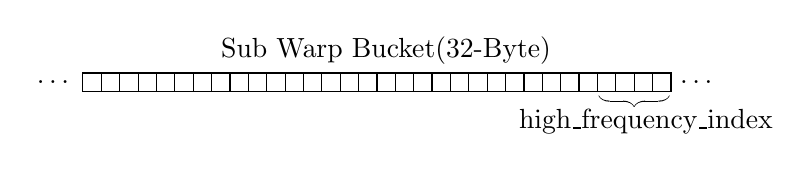
\begin{tikzpicture}[
      start chain=1 going right,start chain=2 going below,node distance=-0.15mm
    %   scale = 0.6
    ]
    \node [on chain=2] at (2.7, 0) {Sub Warp Bucket(32-Byte)};
    \node [on chain=1] at (-1.5,-.4) {\ldots};  
    \foreach \x in {1,2,...,32} {
        \x, \node [draw,on chain=1] {};
        
    } 
    \node [name=r,on chain=1] {\ldots}; 
    \draw [name=b,white,decorate, decoration = {calligraphic brace, raise = 2pt, amplitude = 4pt,mirror}] (5.4,-0.5) --  (6.3,-0.5);
    \node at (6.0,-0.9) {high\_frequency\_index};
\end{tikzpicture}
    \caption{low\_frequency\_bucket}
    \label{fig:low_frequency_bucket}
\end{figure}

The accuracy of sketch is limited by the size of underlying hash tables. A larger hash table usually leads to a more accuracy sketch, because it can store more count variables and each count variable has a lower possibility to be hit by multiple elements, which helps all count variables of an element to be closer to the actual value. Finally, the estimate frequency which is the minimum value of count variables will be closer to the real frequency of the element and the sketch can achieve a high searching accuracy. But the sketch will consume more device memories if it needs a larger hash table. This is not a serious problem for host sketches because a typical server may have 128GB or 256GB host memory, some servers can even install 2TB host memory. However the device memory is usually much smaller than the host memory and it is hard to increase the size of device memory without installing a new GPU. For example, a typical GPU such as NVIDIA Tesla P100 only has 12GB or 16GB device memory and NVIDIA RTX 8000 has 48GB device memory, which is the GPU with the largest device memory, and it is still smaller than the host memory. Some teches[to do: ] and papers\cite{b4} can help the GPU to store the data which is larger than the device memory via using the host memory. But the performance is still limited by the low bandwidth of host memory and PCI Express and it is hard to cache the random access. NVIDIA NVLINK can help one GPU to access the global memory of another GPU and it has a much higher bandwidth than host memory and PCI Express, but it is still lower than the global memory bandwidth of the same GPU. For example, P100 delivers 160 GB/s bidirectional bandwidth in total while it has a peak memory bandwidth of 540 GB/s. Neigher of them can help the GPU to store more count variables without greatly decreasing performance.
Some sketches support to use unsigned character(1-byte integer) as count variable instead of 4-byte integer, which can have 4 times the original variables for the same memory size. However, the maximum value of unsigned character is 255, and it will overflow if there are some elements with have the frequencies higher than 255. And it is still easy to overflow even if the frequencies of all elements are smaller than 255 because different elements may hit the same count variable and the sum of the frequencies of them may be greater than 255.
% for a larger number of elements even the input data is uniform distribution. [to do: 16GB 4-byte counts, 1-byte counts]
% [to do:  prove]
The qsketch\_v3(Level Sketch) uses two hash tables to handle the 1-byte integer overflow problem, which can improve the accuracy without decreasing the performance. Each operation will only need one atomic function or one 32-byte global memory access on average. The first hash table is high\_frequency\_table, which is the same as the hash table of the warp sketch. It will also use 4-byte or 8-byte unsigned integer as its count variables and be stored in global memory. But it is much smaller and the accesses of high\_frequency\_table are easy to be cached in the l2 cache or other fast on-chip caches. A high\_frequency\_table which stores 1024 128-byte high\_frequency\_bucket will only need 128 KB memory and it is much smaller than the L2 cache size of current GPU. For example, Tesla P100 has 4096 KB of L2 cache and 2080ti has 5632 KB of L2 cache.
The second hash table is low\_frequency\_table, which can store a large number of low frequency elements with high accuracy and it will use 1-byte unsigned integer as its count variable. The low\_frequency\_table contains lots of buckets(low\_bucket) and the size of each bucket is 32-byte which can fit in one global memory access. It stores 28 1-byte count variables and the last 4-byte(high\_bucket\_index) of each bucket in the low\_frequency\_table can be used to store an index to the high\_frequency\_table. $0 \sim 1023$ are reserved and $1024 \sim 2 ^ {32} - 1$ are indices. The 4-byte unsigned integer is enough for the size of current device memory, it can support about $2 ^ {32} $ 128-byte high\_frequency\_buckets and the high\_frequency\_table can use up to 512 GB global memory which is much bigger than the largest device memory. Although the low\_frequency\_bucket needs to leave 4 bytes for preventing the overflow problem, it still can have 3.5 times count variables than the buckets with 4-byte integers.
The high\_bucket\_index can also be 3-byte or even 2-byte unsigned integers, and they can support a high\_frequency\_table that is smaller than 2 GB or 8 MB, which is still acceptable for most high\_frequency\_tables and can slightly increase the number of count variables stored in the same size of memory for 3.5 to 3.625 and 3.75. The frequencies of elements in the low\_frequency\_table are usually between 1 and 32. The upper bound may be smaller for a larger low\_frequency\_table because there may be more elements that hit on the same count variable and the maximum value of all count variables should still be less than 255. Both hash tables were allocated and initialized before the first insertion happens. And each sketch object will not share the high\_frequency\_table with others, while they may share the hash mask table. Each hash mask is also 32-bit and the bits for the high\_bucket\_index are always zero. For the 4-byte high\_bucket\_index, it will calculate a normal hash mask of 28-bit and pad 4-bit zero. % explain why
% the same hash mask are used for the low\_bucket and high\_bucket of the same element.
For each insertion of the Level Sketch that each warp contains 4 sub warp and each sub warp has 8 threads, the Level Sketch will load 4 elements, calculate the hash values and load the hash masks, which are similar as the Sub Warp Sketch. Each sub warp has their own element and corresponding low\_bucket and it will load the contents of its low\_bucket by a single global memory access. Then the whole warp will check the values of 4 high\_bucket\_indices via a warp vote function(\_\_any\_sync). If there is at least one of them pointing to a valid high\_frequency\_bucket, the 4 sub warps will merge into a warp and it will check the 4 high\_bucket\_index one by one and insert the element to the high\_frequency\_table if the corresponding high\_bucket\_index is valid. This can save some warp vote functions because it will only need to check all high\_bucket\_indices when there is a low\_bucket that are connected to high\_frequency\_table and the most low\_buckets are unconnected. And the overhead of this step is only a warp vote function for most insertions. The insertion to high\_frequency\_table of each element is similar to the warp sketch insertion and it will need at most 4 32-byte global memory accesses. The actual number of global memory accesses is depend on the hash mask and l2 cache, which are talked in Warp Sketch. If the high\_bucket\_indices are not valid, the sub warps will insert the elements to their own low\_buckets simultaneously, which is also the same as Sub Warp Sketch. 

% However, CUDA doesn't support atomic functions for byte, so the 4 adjacent bytes are combined to a 4-byte integer and the 4 atomic adding are finished together. 
% increment
% Each unsigned byte in low\_bucket is expended to 4-byte or 8-byte unsigned integers in high\_bucket.

But the sub warp will first load the low\_bucket and calculate the maximum value of the count variables within a sub warp. If it is greater than some limits(eg. 128) and the low\_bucket is going to overflow, it won't insert the element to low\_frequency\_table instead of inserting it to high\_frequency\_table. An overflow may still happen if there are more than 127 elements which are inserted at the same time. The sub warps all receive the maximum value less than the limit and then they can insert the elements to low\_frequency\_table and an overflow happens. However this doesn't happen in practice especially when the input data contains millions of the same elements. We have run the test program for more than 100000 times and the unexpected overflow never happens. And an optional function will check if there is an overflow already happened or it is going to happen, if so, it will recall the insertion to the low\_frequency\_table and insert the element to high\_frequency\_table. But it may need extra global memory accesses and atomic functions.
However the low\_buckets may not connect to a valid high\_bucket, each sub warp that needs to insert the element to the high\_frequency\_table but doesn't have a valid high\_bucket\_index will invoke an atomicMalloc() to link a low\_bucket to a high\_bucket. The first thread of each sub warp will be responsible for the atomicMalloc(), and it will first use an atomic compare and swap function(Line :7 of atomic allocate algorithm). If the old value of high\_bucket\_index is 0, this warp or sub warp will set the high\_bucket\_index to 1 and it will request an available bucket(high\_bucket) in the high\_frequency\_table via an atomicAdd()(Line :9 of atomic allocate algorithm). The next\_level\_id is a global variable and its initial value is 1025 which can make sure the atomicAdd() will always return a valid high\_bucket\_index. Then it will also store the index of the new bucket to the high\_bucket\_index of corresponding low\_bucket(high\_bucket\_index). If the old value of high\_bucket\_index is non zero, there must be another thread working on the allocation, those sub warps only need to wait in a busy loop, and they won't wait for a long time because the atomic allocation only needs to invoke an atomic increase function and write the data to global memory, and there is no real memory allocation. \_\_ldcv() is load function with cache hint, it will load the values in the global memory and it can be replaced with keyword volatile. \_\_threadfence\_block() is needed because the global memory is weakly-ordered and it can make sure the allocating thread read data in order so it will always get the correct index. Without threadfence function, the sketch may read some incorrect indices every 5000 runs. Those atomic allocations won't happen frequently for most situation. It only invokes 3 or 5 atomic allocations while inserting 1 million elements to a sketch. The overhead of atomic allocation is trivial for the sketch insertion algorithm. After the atomic allocation, the 4 sub warps will merge into a warp and insert the element into high\_frequency\_table. They are the same as if they read the valid high\_bucket\_index at the beginning of insertion. The Level Sketch will reuse the high\_buckets when it runs out of high\_frequency\_table by calculating $(high\_bucket\_index - 1024) mod high\_frequency\_table\_size$. It can also increase the size of high\_frequency\_table by reallocating but it will greatly reduce the performance and should only be used for debugging or detecting a suitable size of high\_frequency\_table. A fast and dynamic high\_frequency\_table is meaningless, because if the overflow happens frequently and the high\_frequency\_table is much larger than expected, then the high\_frequency\_table may not be well cached and it will reduce the overall performance. At this situation, users can chose one level sketch such as Sub Warp Sketch instead. For most insertions, there is no need to take care of high\_bucket\_index, it only needs to insert the element to low\_frequency\_table. However, CUDA doesn't support atomic functions for byte, so the 4 adjacent bytes are combined to a 4-byte integer and the 4 atomic operations are finished together. 

For searching, if the low\_bucket is not linked to any high\_bucket, it only need to calculate and return the minimum value of low\_bucket. Each thread will load 4-byte data, then split it into 4 1-byte integers and calculate the minimum value within the thread. The sub warps will calculate their own minimum value via sub warp reduce function. The value(EFL) is the estimated frequency of the element stored in low\_frequency\_table, the first thread of each sub warp will write it to result array. But if a low\_bucket is already linked to a high\_bucket, it needs to calculate the EFL. Then it also needs to the estimated value(EFH) of the connected high\_bucket, which is the estimated frequency of the element stored in high\_frequency\_table. The 4 sub warps merge into a warp and it will check the 4 high\_bucket\_index one by one and calculate the minimum value of the high\_frequency\_table if the corresponding high\_bucket\_index is valid. The sub warp reduce functions of EFL and warp reduce functions of EFH are calculated separately and then add them together to get the estimated frequency of the element. This can help to increase the accuracy without decreasing the performance. For three arrays with the same length, $A$, $B$ and $C$ where $c_i = a_i + b_i$. There is always $min(A) + min(B) <= min(C)$ because the minimum values of A and B may not in the same place and if so, all values in $C$ are greater than $min(A) + min(B)$. The accuracy of two separate minimum values should be higher than the accuracy of migrating the data from low\_bucket to the corresponding high\_bucket. And another reason is that the two buckets use more memories than one high\_bucket and it has a higher memory utilization and accuracy. It needs 4 extra 32-byte global memory accesses but most of them are well cached in the l2 cache and only a few elements need to access high\_bucket, so this won't decrease the searching performance greatly.
If a low frequency element($L$) and a high frequency element($H$) are inserted to the same low\_bucket by accidentally and the low\_bucket has already been connected to a high\_bucket, it seems that the accuracy of $L$ may be much greater than the real value due to the influence of $H$, although the frequency of $L$ is low and it has never been inserted to high\_bucket. However this can be prevented because they usually have different hash\_masks and there is at least one different bit, and the smallest value of count variables in high\_bucket for $L$ may be still 0. But if they select the same low\_bucket and hash mask or other high frequency elements increase the count variables of $L$, the estimate value of $L$ will be much greater than the real value. So, users should carefully chose the hash functions of for bucket and mask so that they are independent. And they can also increase the size of hash table so it can store enough hash masks to avoid those collisions, especially when the sketches are running on device with large l2 cache or fast caches. If they run several sketches at the same time, those sketch can share a large hash mask table without using their own small hash mask table, which can increase the accuracy without decreasing performance. 


\begin{algorithm}
    \DontPrintSemicolon
    \caption{atomic allocate algorithm}
    \SetKwProg{Fn}{Function}{}{end}
    \SetKw{KwRet}{return}
    \SetKw{Kwin}{in}
    \SetKw{KwStep}{step}
    \SetKwFunction{FnInsert}{insert}
    \SetKwFunction{FnSearch}{search}
    $table[p * w] \longleftarrow 0$\;
    $mask\_table[H]$\;
    % s : the elements each warp loads
    $s \longleftarrow the elements each warp loads$\;
    $sub\_warp\_size = warp\_size / s $\;
    \SetKwFor{ParallelForEach}{parallel for each}{do}{endfor}
    \SetKwFunction{FnAtomicAllocate}{atomicAllocate}
\Fn(){\FnAtomicAllocate{high\_bucket\_index, global\_index}}
{
    $id \leftarrow 0$\;
    $old \leftarrow atomicCAS(high\_bucket\_index, 0, 1)$\;
    \If{$old == 0$}{
        $id \leftarrow atomicAdd(global\_index, 1)$\;
        $high\_bucket\_index \leftarrow id\;$
    }
    \Else {
        \While{$id <= 1$}{
            $id$ $\leftarrow$ max($id$, \_\_ldcv(high\_bucket\_index))\;
            \_\_threadfence\_block()\;
        }
    }
    \KwRet id\;
}
\end{algorithm}

\subsection{Host Supported Sketch}

\begin{algorithm}
    \DontPrintSemicolon
    \caption{Host Supported Sketch algorithm}
    \SetKwProg{Fn}{Function}{}{end}
    \SetKw{KwRet}{return}
    \SetKw{Kwin}{in}
    \SetKw{KwStep}{step}
    \SetKwFunction{FnInsert}{insert}
    \SetKwFunction{FnSearch}{search}
    $\_device\_ d\_table[p * w] \longleftarrow 0$\;
    $\_host\_ h\_table[p * w * n] \longleftarrow 0$\;
    $device\_mask\_table[H]$\;
    $host\_mask\_table[H]$\;
    $s \longleftarrow the elements each warp loads$\;
    $sub\_warp\_size = warp\_size / s $\;
    \SetKwFor{HostParallelForEach}{parallel for each}{do}{endfor}
\Fn(){\FnInsert{keys}}
{
    \HostParallelForEach{$key$ \Kwin $keys$}
    {
        $hv \leftarrow hash(key)$\;
        $id \leftarrow hv \% p$\;
        $sub\_bucket\_id[w] \leftarrow mask\_table[hv \% H]$\;
        \For{$i\leftarrow 0$ \KwTo $w$, \KwStep $1$}
        {
            $sbi \leftarrow sub\_bucket\_id[i]$\;
            $sub\_bucket \leftarrow h\_table[id][sbi]$\;
            $jd \leftarrow hash(key, i) \% n$\;
            atomic\_add($sub\_bucket[jd], 1$)\;
            device\_update($sub\_bucket$);
        }
    }
}
\end{algorithm}

For many users, the searching performance is much more important than the insertion and deleting performance. And many clusters or servers also have a large unused host memory, while running the sketches on GPU.  The Host Supported Sketch can use the host memory to improve the accuracy without losing the searching performance. This idea was inspired by SF-sketch\cite{b3}, which improves the accuracy by using two sketches table. It also uses two hash tables, one for insertion and deleting which is large and in host memory. The other one is for searching, which is relative small and in device memory.
For example, the device hash table has $p$ buckets and each bucket has $w$ count variables. The host hash table is $n$ times larger than the device hash table, it has $p$ buckets but each bucket has $w$ sub bucket. Each sub bucket has $n$ count variable. Each count variables in device hash table is the maximum value of $n$ count variables of a sub bucket in the host hash table. The Host Supported sketch also has a host hash mask table, which is exactly same as the device one. Actually the hash mask table is generated on host, this sketch will keep it after copying it to device.
The sketch execute insertion and deletion on host side. It first calculates a hash value then selects a bucket and hash mask according to the hash value. It will update one random count variable of the sub buckets if the bits for those sub buckets in the hash mask are 1. The random count variable of the sub bucket can also be selected by the hash value in first step. So it still needs one hash function for each operation. After if finishes the operation, it will copy the $n$ count variables to the device memory. The device will calculate the maximum value of $n$ variables then update its device count variable. The performance of insertion and deleting is limited by computing power and memory bandwidth of CPU, and it should be much lower than the Sub Warp Sketch. And the insertion and deletion performance may also be limited by the bandwidth of PCI Express, so the host can calculate the maximum value and compare it with the old maximum value. It only copy the new value to the device for each insertion or deletion when the value is actually changed. But the performance of host insertion and deletion will still be slow.
The searching method is exactly same as what the Sub Warp Sketch does, so the searching performance is unchanged.
\section{results}
% platform
% 2080ti, tesla p100

% We evaluate our slab list and slab hash on an NVIDIA Tesla K40c GPU (with ECC disabled), which has a Kepler microarchitecture with compute capability of 3.5, 12 GB of GDDR5 memory, and a peak memory bandwidth of 288 GB/s.
%for insertion, ideally we will have one memory access (reading the slab) and a single atomicCAS to insert into an empty lane. For search, it will be a single memory access plus some overhead from extra warp-wide instructions (Section IV).

% P100 has 12GB HBM2 memory and memory bandwidth 540 GB/s, with Compute Capability 6.0.
% 2080ti 11GB GDDR6 memory and 616 GB/s memory bandwidth, with Compute Capability 7.5.


% cuda 11, Compute Capability 6.0, 7.5
% grid size, maximum performance
% compare it with example one random memory access algorithm,
% a1: thread sketch [m = 1], higher l2 cache hit rate
% a2: hash table, slabhash and other hash table
% relative error
% We use relative error (RE) to quantify the accuracy of sketches. Let fe represent the actual frequency of an item e
% nd let fe represent the estimate of the frequency returned by the sketch, the relative error is defined as the ratio |fˆ −f |/f .
We evaluate qsketch on both NVIDIA Tesla P100 and Nvidia GeForce RTX 2080 Ti. 
The P100 has a Pascal architecture with Compute Capability 6.0 and 12GB HBM2 memory(with ECC enabled), which can achieve a peak memory bandwidth of 540 GB/s. It is a computing processor and widely used on high-performance computing clusters. The 2080ti has a Turing architecture with Compute Capability of 7.5 and 11GB GDDR6 memory(it doesn't support ECC), and the peak memory bandwidth of it is 616 GB/s, which is slightly higher than p100. We compile the codes with CUDA 11 and run the program with a large range of grid size($1024 \sim 2 ^ {23}$) to get the peak performance. We test the qsketch for 10 batches and each batch runs the test code more than 50 times. And we only record the best performance of each batch for p100 because the p100 is installed on cluster and the node may be shared by other users. The final results are the average of all best performance of each batch. We claims that the qsketch only needs a single coalesced atomic access for each insertion on average and it also needs only one global memory access for each searching on average. So we compare the performance of qsketch with other algorithms which also need only one atomic access or global memory access for each operation. The thread sketch$(m = 1)$ which are inserted with uniform keys should be the fastest one since each insertion only needs one atomic increase operation and one 4-byte read operation for each searching. It doesn't need any hash functions or warp instructions and there is no extra overhead except the sequential reading of input keys. We also compare the performance with hash tables, such as SlabHash,[to do: add more hash table algorithms]. Those hash tables also need one random atomic operation or global memory access for each operation. And we compare the accuracy of qsketch with other sketch algorithms, which are only implemented on CPU platform. We also use the relative error(RE) to quantify the accuracy of sketches\cite{b3}. The relative error is $\lvert e - a \rvert / a$, where $e$ is the estimate value of frequency and $a$ is the actual value.
% grid size
% generate random keys
We test the qsketch with several different distributions of random keys and real data set. The time usages of generating random keys, loading real data set from disk and transferring data between host and device are not calculated in the performance. The random keys of uniform distribution are generated by curand on device and the others are generated or loaded by host functions. The input keys are grouped into batches so they can fit in a device buffer, and the batches may execute simultaneously or sequentially. We also test different buffer size($2 \sim 128 MB$) and we find $64 MB$ buffer is enough for most situations. 

% host random keys, other data set
% batch size

% work load factor
% frequency test

The work load is highly related to the performance and accuracy. We test the qsketch for different work load factor(WLF). 
\[WLF = \frac{inserted\_keys * increments\_per\_key}{total\_count\_variables}\]. 

\subsection{Performance}
% explain figures

% generate random input
% real data set
% 1. random test
% 2. frequency test
% performance vs bandwidth
% batch size
% mix insert and search bench
% l2 cache hit rate

% large object 
Figure \ref{fig:insert_perf_sketch_2080ti_0.5} and Figure \ref{fig:insert_perf_sketch_2080ti_1} show the insertion performance of 4 sketches on 2080ti. For small data, insertion performance improves as the work load expands. Because if there are not enough insertion keys, some SMs will idle and the overall performance will be low. For a small input data set, the hash tables in sketches are also small because the workload factor is a constant number. The most of count variables are cached in the l2 cache, so there is a higher l2 cache hit rate for the small input data set. The sketches are not limited be the memory throughput, and Thread Sketch, Warp Sketch, Sub\_Warp Sketch and Multi\_Level Sketch have an increasing computational workload, which leads to decreasing insertion performance. The insert performance of Thread Sketch greatly decreases as the workload increases because it runs out of l2 cache and the l2 cache hit rate is low. The most memory accesses are not cached and the Thread Sketch is limited by the random access performance of global memory. The insertion performance of Warp Sketch is approximately three times that of Thread Sketch, which means that Warp Sketch successfully coalesced three global memory accesses into one. 
% The atomic function are compiled into ATOM or RED instructions. The ATOM will return the old value while RED won't,  
% Figure \ref{fig:search_perf_sketch_2080ti_0.5} and Figure \ref{fig:search_perf_sketch_2080ti_1} 
show the searching performance of 4 sketches. The behaviors of Thread Sketch and Sub Warp Sketch are similar as the insertion, while the searching performance of Warp Sketch is only slightly higher than Thread Sketch. The reason is that the Warp Sketch only needs to read 3 count variables but they are evenly split across in a 128-byte bucket. They still need 3 32-byte global memory accesses for most insertions. For the Sub Warp Sketch, the 3 variables are in a 32-byte bucket and they can be coalesced into one 32-byte memory. 
% RED instruction and ATOM
\begin{figure}
    \centering
    \subfloat[2080ti, WLF = 0.5\label{insert_2080ti_0.5}]{
        \resizebox{0.48\columnwidth}{!}{
            \begin{tikzpicture}[scale = 0.48]
    \label{fig:insert_perf_sketch_2080ti_0.5}
    \begin{semilogxaxis}[
        % title={Insert Performance(WLF = 0.5)},
        xlabel={Work Load},
        ylabel={Insert Performance (M operations/s)},
        legend pos=north east,
        xmajorgrids=true,
        ymajorgrids=true,
    ]
        \addplot table[x = WorkLoad, y = ThreadInsert] {data/qsketch/perf_2080ti_0.5.dat};
        \addlegendentry{Thread Insert}
        \addplot table[x = WorkLoad, y = WarpInsert] {data/qsketch/perf_2080ti_0.5.dat};
        \addlegendentry{Warp Insert}
        \addplot table[x = WorkLoad, y = Sub_WarpInsert] {data/qsketch/perf_2080ti_0.5.dat};
        \addlegendentry{Sub\_Warp Insert}
        \addplot table[x = WorkLoad, y = LevelInsert] {data/qsketch/perf_2080ti_0.5.dat};
        \addlegendentry{Level Insert}
    \end{semilogxaxis}
\end{tikzpicture}
        }
    }
    ~
    \hfill
    \subfloat[2080ti, WLF = 1.0\label{insert_2080ti_1.0}]{
        \resizebox{0.48\columnwidth}{!}{
            \begin{tikzpicture}[scale = 0.48]
    \label{fig:insert_perf_sketch_2080ti_1}
    \begin{semilogxaxis}[
        % title={Insert Performance(WLF = 1.0)},
        xlabel={Work Load},
        ylabel={Insert Performance (M operations/s)},
        legend pos=north east,
        xmajorgrids=true,
        ymajorgrids=true,
    ]
        \addplot table[x = WorkLoad, y = ThreadInsert] {data/qsketch/perf_2080ti_1.0.dat};
        \addlegendentry{Thread Insert}
        \addplot table[x = WorkLoad, y = WarpInsert] {data/qsketch/perf_2080ti_1.0.dat};
        \addlegendentry{Warp Insert}
        \addplot table[x = WorkLoad, y = Sub_WarpInsert] {data/qsketch/perf_2080ti_1.0.dat};
        \addlegendentry{Sub\_Warp Insert}
        \addplot table[x = WorkLoad, y = LevelInsert] {data/qsketch/perf_2080ti_1.0.dat};
        \addlegendentry{Level Insert}
    \end{semilogxaxis}
\end{tikzpicture}
        }
    }
    
    \subfloat[p100, WLF = 0.5\label{insert_p100_0.5}]{
        \resizebox{0.48\columnwidth}{!}{
            \input{graphs/insert_perf_p100_0.5}
        }
    }
    ~
    \hfill
    \subfloat[p100, WLF = 1.0\label{insert_p100_1.0}]{
        \resizebox{0.48\columnwidth}{!}{
            \input{graphs/insert_perf_p100_1.0}
        }
    }
    \caption{Insert Performance}
    \label{fig:insert_performance}
\end{figure}

\begin{figure}
    \centering
    \subfloat[2080ti, WLF = 0.5\label{search_2080ti_0.5}]{
        \resizebox{0.48\columnwidth}{!}{
            \begin{tikzpicture}[scale = 0.48]
    \label{fig:search_perf_sketch_2080ti_0.5}
    \begin{semilogxaxis}[
        % title={Search Performance},
        xlabel={Work Load},
        ylabel={Search Performance (M operations/s)},
        legend pos=north east,
        xmajorgrids=true,
        ymajorgrids=true,
    ]
        \addplot table[x = WorkLoad, y = ThreadSearch] {data/qsketch/perf_2080ti_0.5.dat};
        \addlegendentry{Thread Search}
        \addplot table[x = WorkLoad, y = WarpSearch] {data/qsketch/perf_2080ti_0.5.dat};
        \addlegendentry{Warp Search}
        \addplot table[x = WorkLoad, y = Sub_WarpSearch] {data/qsketch/perf_2080ti_0.5.dat};
        \addlegendentry{Sub\_Warp Search}
        \addplot table[x = WorkLoad, y = LevelSearch] {data/qsketch/perf_2080ti_0.5.dat};
        \addlegendentry{Level Search}
    \end{semilogxaxis}
\end{tikzpicture}
        }
    }
    ~
    \hfill
    \subfloat[2080ti, WLF = 1.0\label{search_2080ti_1.0}]{
        \resizebox{0.48\columnwidth}{!}{
            \input{graphs/search_perf_2080ti_1.0}
        }
    }
    
    \subfloat[p100, WLF = 0.5\label{search_p100_0.5}]{
        \resizebox{0.48\columnwidth}{!}{
            \input{graphs/search_perf_p100_0.5}
        }
    }
    ~
    \hfill
    \subfloat[p100, WLF = 1.0\label{search_p100_1.0}]{
        \resizebox{0.48\columnwidth}{!}{
            \begin{tikzpicture}[scale = 0.48]
    \label{fig:search_perf_sketch_p100_1}
    \begin{semilogxaxis}[
        % title={Search Performance},
        xlabel={Work Load},
        ylabel={Search Performance (M operations/s)},
        legend pos=north east,
        xmajorgrids=true,
        ymajorgrids=true,
    ]
        \addplot table[x = WorkLoad, y = ThreadSearch] {data/qsketch/perf_p100_1.0.dat};
        \addlegendentry{Thread Search}
        \addplot table[x = WorkLoad, y = WarpSearch] {data/qsketch/perf_p100_1.0.dat};
        \addlegendentry{Warp Search}
        \addplot table[x = WorkLoad, y = Sub_WarpSearch] {data/qsketch/perf_p100_1.0.dat};
        \addlegendentry{Sub\_Warp Search}
        \addplot table[x = WorkLoad, y = LevelSearch] {data/qsketch/perf_p100_1.0.dat};
        \addlegendentry{Level Search}
    \end{semilogxaxis}
\end{tikzpicture}
        }
    }
    \caption{Search Performance}
    \label{fig:search_performance}
\end{figure}

% \begin{tikzpicture}[scale = 0.48]
    \label{fig:insert_perf_sketch_2080ti_0.5}
    \begin{semilogxaxis}[
        % title={Insert Performance(WLF = 0.5)},
        xlabel={Work Load},
        ylabel={Insert Performance (M operations/s)},
        legend pos=north east,
        xmajorgrids=true,
        ymajorgrids=true,
    ]
        \addplot table[x = WorkLoad, y = ThreadInsert] {data/qsketch/perf_2080ti_0.5.dat};
        \addlegendentry{Thread Insert}
        \addplot table[x = WorkLoad, y = WarpInsert] {data/qsketch/perf_2080ti_0.5.dat};
        \addlegendentry{Warp Insert}
        \addplot table[x = WorkLoad, y = Sub_WarpInsert] {data/qsketch/perf_2080ti_0.5.dat};
        \addlegendentry{Sub\_Warp Insert}
        \addplot table[x = WorkLoad, y = LevelInsert] {data/qsketch/perf_2080ti_0.5.dat};
        \addlegendentry{Level Insert}
    \end{semilogxaxis}
\end{tikzpicture}
% ~
% \begin{tikzpicture}[scale = 0.48]
    \label{fig:insert_perf_sketch_2080ti_1}
    \begin{semilogxaxis}[
        % title={Insert Performance(WLF = 1.0)},
        xlabel={Work Load},
        ylabel={Insert Performance (M operations/s)},
        legend pos=north east,
        xmajorgrids=true,
        ymajorgrids=true,
    ]
        \addplot table[x = WorkLoad, y = ThreadInsert] {data/qsketch/perf_2080ti_1.0.dat};
        \addlegendentry{Thread Insert}
        \addplot table[x = WorkLoad, y = WarpInsert] {data/qsketch/perf_2080ti_1.0.dat};
        \addlegendentry{Warp Insert}
        \addplot table[x = WorkLoad, y = Sub_WarpInsert] {data/qsketch/perf_2080ti_1.0.dat};
        \addlegendentry{Sub\_Warp Insert}
        \addplot table[x = WorkLoad, y = LevelInsert] {data/qsketch/perf_2080ti_1.0.dat};
        \addlegendentry{Level Insert}
    \end{semilogxaxis}
\end{tikzpicture}
% \begin{tikzpicture}[scale = 0.48]
    \label{fig:search_perf_sketch_2080ti_0.5}
    \begin{semilogxaxis}[
        % title={Search Performance},
        xlabel={Work Load},
        ylabel={Search Performance (M operations/s)},
        legend pos=north east,
        xmajorgrids=true,
        ymajorgrids=true,
    ]
        \addplot table[x = WorkLoad, y = ThreadSearch] {data/qsketch/perf_2080ti_0.5.dat};
        \addlegendentry{Thread Search}
        \addplot table[x = WorkLoad, y = WarpSearch] {data/qsketch/perf_2080ti_0.5.dat};
        \addlegendentry{Warp Search}
        \addplot table[x = WorkLoad, y = Sub_WarpSearch] {data/qsketch/perf_2080ti_0.5.dat};
        \addlegendentry{Sub\_Warp Search}
        \addplot table[x = WorkLoad, y = LevelSearch] {data/qsketch/perf_2080ti_0.5.dat};
        \addlegendentry{Level Search}
    \end{semilogxaxis}
\end{tikzpicture}
% ~
% \input{graphs/search_perf_2080ti_1.0}

The insertion and searching performance of qsketch are close to the performance of example one random memory access algorithms, such as Thread Sketch(m = 1) and hash tables. But the qsketch is still slower than them, because those algorithms only need to access 4 or 8 bytes global memory for each operation, while the Warp Sketch and Sub Warp Sketch need to access 32 or more bytes for each operation. The cache can store more variables for those algorithms and they will experience a higher l2 cache hit rate as if they have a 4 times larger l2 cache.
% \input{graphs/insert_perf_p100_0.5}
% ~
% \input{graphs/insert_perf_p100_1.0}
% \input{graphs/search_perf_p100_0.5}
% ~
% \begin{tikzpicture}[scale = 0.48]
    \label{fig:search_perf_sketch_p100_1}
    \begin{semilogxaxis}[
        % title={Search Performance},
        xlabel={Work Load},
        ylabel={Search Performance (M operations/s)},
        legend pos=north east,
        xmajorgrids=true,
        ymajorgrids=true,
    ]
        \addplot table[x = WorkLoad, y = ThreadSearch] {data/qsketch/perf_p100_1.0.dat};
        \addlegendentry{Thread Search}
        \addplot table[x = WorkLoad, y = WarpSearch] {data/qsketch/perf_p100_1.0.dat};
        \addlegendentry{Warp Search}
        \addplot table[x = WorkLoad, y = Sub_WarpSearch] {data/qsketch/perf_p100_1.0.dat};
        \addlegendentry{Sub\_Warp Search}
        \addplot table[x = WorkLoad, y = LevelSearch] {data/qsketch/perf_p100_1.0.dat};
        \addlegendentry{Level Search}
    \end{semilogxaxis}
\end{tikzpicture}

% Figure \ref{fig:insert_perf_sketch_p100_0.5}, Figure \ref{fig:insert_perf_sketch_p100_1}, Figure \ref{fig:search_perf_sketch_p100_0.5} and Figure \ref{fig:search_perf_sketch_p100_1} 
show the performance of qsketch running on Tesla P100. 2080ti and P100 have different device memories, 2080t1 has 11 GB GDDR6 memory while P100 has 12 GB HBM2. And the memory bandwidth of P100 is 540GB/s which is $87.7\%$ of the bandwidth of 2080ti, and the searching performance of P100 is also about $87.7\%$ of 2080ti. This also shows that the searching performance is highly related to the global memory bandwidth. The performance of Warp Sketch is different for two GPUs, it runs slower on P100 compared to others.
The Level Sketch is also slightly slower than Sub Warp Sketch on P100. Because the Level Sketch has a relatively heavier computing overhead compared to Sub Warp Sketch and the computing power of P100 is also relative slower. The 2080ti has 14 TFLOPs and P100 has 10 TFLOPs. The peak FLOPs of P100 is only about $71.4\%$ of 2080ti, so the ratio of computing power and memory bandwidth of P100 is smaller than that of 2080ti.


% \subsection{Insertion Speed}
% \subsection{Deletion Speed}
% \subsection{Searching Speed}
\subsection{Accuracy}
% deleted: isolated accuracy and speed test
The actual frequencies of element are stored in hash table in the host memory and they will be copied to device memory when needed because the device memory may not be enough to store a large input data set. The Thread Sketch, Warp Sketch, and Sub\_Warp Sketch have an decreasing accuracy because the size of bucket is going smaller and the count variables of an element in Warp Sketch and Sub\_Warp Sketch will become much more concentrated than that of Thread Sketch. The hash functions of Warp Sketch and Sub Warp Sketch work like one of the three hash functions of Thread Sketch, but the thread sketch also have another two hash functions which are independent and mapped into a large area. So the possibility for that all count variables of an element have Collisions with others is low. But the Warp Sketch and Sub Warp Sketch can only select a random hash mask based on the previous hash value for selecting buckets. The total number of hash masks is much smaller than the size of a normal hash table if the program want to have a high l2 cache hit rate and high performance, so the hash masks have a relatively high probability of collision. And even if different hash masks are selected, the count variables within a bucket still have a high collision probability for the small size of bucket. The Multi Level Sketch outperforms because it can have more count variables while using the same size of device memory.

\begin{figure}
    \centering
    \subfloat[WLF = 0.5\label{accuracy_0.5}]{
        \resizebox{0.48\columnwidth}{!}{
            \begin{tikzpicture}[scale = 0.48]
    \begin{semilogxaxis}[
        % title={Accuracy (Load Factor = 0.5)},
        xlabel={Memory Usage},
        ylabel={Accuracy (\%)},
        legend pos=north east,
        xmajorgrids=true,
        ymajorgrids=true,
    ]

        \addplot table[x = ThreadMemoryUsage, y = Thread] {data/qsketch/accuracy_0.5.dat};
        \addlegendentry{Thread}
        \addplot table[x = WarpMemoryUsage, y = Warp] {data/qsketch/accuracy_0.5.dat};
        \addlegendentry{Warp}
        \addplot table[x = Sub_WarpMemoryUsage, y = Sub_Warp] {data/qsketch/accuracy_0.5.dat};
        \addlegendentry{Sub\_Warp}
        \addplot table[x = Sub_Warp_LevelMemoryUsage, y = Sub_Warp_Level] {data/qsketch/accuracy_0.5.dat};
        \addlegendentry{Level}
    \end{semilogxaxis}
\end{tikzpicture}
        }
    }
    ~
    \hfill
    \subfloat[WLF = 1.0\label{accuracy_1.0}]{
        \resizebox{0.48\columnwidth}{!}{
            \begin{tikzpicture}[scale = 0.48]
    \begin{semilogxaxis}[
        % title={Accuracy (Load Factor = 1.0)},
        xlabel={Memory Usage},
        ylabel={Accuracy (\%)},
        legend pos=north east,
        xmajorgrids=true,
        ymajorgrids=true,
    ]

        \addplot table[x = ThreadMemoryUsage, y = Thread] {data/qsketch/accuracy_1.0.dat};
        \addlegendentry{Thread}
        \addplot table[x = WarpMemoryUsage, y = Warp] {data/qsketch/accuracy_1.0.dat};
        \addlegendentry{Warp}
        \addplot table[x = Sub_WarpMemoryUsage, y = Sub_Warp] {data/qsketch/accuracy_1.0.dat};
        \addlegendentry{Sub\_Warp}
        \addplot table[x = Sub_Warp_LevelMemoryUsage, y = Sub_Warp_Level] {data/qsketch/accuracy_1.0.dat};
        \addlegendentry{Level}
    \end{semilogxaxis}
\end{tikzpicture}
        }
    }
    \caption{Accuracy}
    \label{fig:accuracy}
\end{figure}

\section{conclusion}

\begin{thebibliography}{00}
\bibitem{b1} NVIDIA Corporation, “NVIDIA CUDA C++ programming guide,” 2021, version 11.0.
\bibitem{b2} NVIDIA Corporation, “NVIDIA CUDA C++ programming guide,” 2021, version 11.0.
\bibitem{b3} L. Liu et al., "SF-Sketch: A Two-Stage Sketch for Data Streams," in IEEE Transactions on Parallel and Distributed Systems, vol. 31, no. 10, pp. 2263-2276, 1 Oct. 2020, doi: 10.1109/TPDS.2020.2987609.
\bibitem{b4} Compiler Assisted Hybrid Implicit and Explicit GPU Memory Management under Unified Address Space % not found in IEEE
% Lingda Li and Barbara Chapman. 2019. Compiler assisted hybrid implicit and explicit GPU memory management under unified address space. In Proceedings of the International Conference for High Performance Computing, Networking, Storage and Analysis (SC '19). Association for Computing Machinery, New York, NY, USA, Article 51, 1–16. DOI:https://doi.org/10.1145/3295500.3356141
\bibitem{b5} S. Ashkiani, M. Farach-Colton and J. D. Owens, "A Dynamic Hash Table for the GPU," 2018 IEEE International Parallel and Distributed Processing Symposium (IPDPS), 2018, pp. 419-429, doi: 10.1109/IPDPS.2018.00052.


% \bibitem{}
\end{thebibliography}

\end{document}
